\chapter{Lecture 16 - Fourier Series}
\label{ch:lec16}
\section{Objectives}
\begin{itemize}
\item Review trigonometric series.
\item Derive/show the formulas for expansion of a function as a trigonometric (Fourier) series.
\item Discuss periodic extensions of non-periodic functions, sine/cosine expansions, and convergence behavior.
\end{itemize}

\section{Review of Fourier Series}
In the last lecture we learned about orthogonal functions and sets of orthogonal functions.  We stated that most any function can be expressed as a linear combination of those orthogonal functions:
\begin{equation*}
u(x) = \sum\limits_{n=0}^{\infty} c_n \phi_n
\end{equation*}
where $\phi_n$ are members of a set of orthogonal functions and $c_n$ are determined by:
\begin{equation*}
c_n = \frac{(u,\phi_n)}{||\phi_n||^2}
\end{equation*} \index{Fourier Series}
You should already have experience with expansions such as this from your previous classes in differential equations in the form of Fourier series expansions.  In that case the orthogonal functions, $\phi_n(x)$, were:
\begin{equation*}
\left\{1,\cos{\frac{\pi x}{p}},\cos{\frac{2\pi x}{p}},\dots,\sin{\frac{\pi x}{p}}, \sin{\frac{2\pi x}{p}}, \dots \right\}
\end{equation*}
\marginnote[-1.5cm]{The function $\phi(x) = 1$ could also be written: $\cos{\frac{0 \pi x}{p}}$.}where $p$ indicates the \emph{period}.\sidenote[][-0.5cm]{Reminder that a function, $f(x)$, is periodic with period $p$ if $f(x+p) = f(x)$.} 

It can be directly shown that members of this set of functions are all mutually orthogonal.  We will demonstrate this for the members of the form $\phi_n(x) = \cos{\sfrac{n \pi x}{p}}$; other cases are left for homework exercises.

\vspace{1.0cm}

\noindent\textbf{Example:} Show that functions of the form $\phi_n(x) = \cos{\frac{n\pi x}{p}}$ are orthogonal over the interval $x \in [-p,p]$:

\vspace{0.5cm}
\noindent Consider two functions, $\phi_n(x)$ and $\phi_m(x)$ where $m,n$ are integers and $m \ne n$.  The functions are orthogonal on the interval $x\in [-p,p]$ if $(\phi_n,\phi_m) = 0$.  From the definition of the inner product:\marginnote[0.5cm]{Here we use the identity: $\cos{(\alpha \pm \beta)} = \cos{\alpha}\cos{\beta} \mp \sin{\alpha}\sin{\beta}$. So that:
\begin{align*}
\cos{\left(\alpha + \beta\right)} &= \cos{\alpha}\cos{\beta} - \sin{\alpha}\sin{\beta} \\
+\cos{\left(\alpha - \beta\right)} &= \cos{\alpha}\cos{\beta} + \sin{\alpha}\sin{\beta} \\
&= 2\cos{\alpha}\cos{\beta}
\end{align*}
and therefore:
\begin{align*}
\cos{\alpha}\cos{\beta} &= \frac{1}{2}\left[\cos{\left(\alpha + \beta\right)} + \cos{\left(\alpha - \beta\right)}\right].
\end{align*}
}
\begin{align*}
(\phi_n,\phi_m) &= \int_{-p}^{p} \cos{\frac{n \pi x}{p}} \cos{\frac{m \pi x}{p}} \ dx \\
&= \frac{1}{2}\int_{-p}^{p} \cos{(n+m)\frac{\pi x}{p}} + \cos{(n-m)\frac{\pi x}{p}} \ dx \\
&= \frac{1}{2} \left[\frac{1}{n+m} \frac{p}{\pi}\sin{(n+m)\frac{\pi x}{p}}\Bigl|_{-p}^{p} + \frac{1}{n-m}\frac{p}{\pi}\sin{(n-m)\frac{\pi x}{p}}\Bigl|_{-p}^{p} \right] \\
&=0
\end{align*}
where the last terms are zero since we are evaluating the sine function at integer multiples of $\pi$.  This shows, at least, all of the cosine members are orthogonal.  For the case $m=n$ we get:\marginnote[1.0cm]{Rather than derive this rigorously, we will combine a tabulated result of standard integrals: $\int \cos^2 u \ du = \frac{1}{2}u + \frac{1}{4}\sin{2u}+C$, with $u$ substitution.}
\begin{align*}
\left(\phi_n,\phi_n \right) &= \int_{-p}^{p} \cos{\left(\frac{n \pi x}{p} \right)}^2 \\
&= \frac{p}{n \pi} \left[\frac{1}{2}\frac{n \pi x}{p} + \frac{1}{4} \sin{\frac{2 n \pi x}{p}} \right]\Bigl|_{-p}^{p} \\
&= \frac{p}{2} - \frac{-p}{2} \\
&= p
\end{align*}

\newthought{We can use} this infinite set of orthogonal functions to represent (nearly) any other continuous function over the interval $[-p,p]$.\marginnote{You might be wondering at this point why you would ever want to represent a function $f(x)$ as a linear combination of orthogonal functions.  The answer is that the members of the set of orthogonal functions are solutions to a linear homogeneous boundary value problem and the function $f(x)$ will be a boundary condition for a partial differential equation that we are trying to solve.}  In your differential equations class you did this by using Equation \ref{eq:fourier-exp}:

\begin{equation}
f(x) = \frac{a_0}{2} + \sum\limits_{n=1}^{\infty}\left[a_n \cos{\frac{n \pi x}{p}} + b_n \sin{\frac{n \pi x}{p}} \right]
\label{eq:fourier-exp}
\end{equation}
We can solve for the coefficients $a_0$, $a_n$ and $b_n$ one at a time by multiplying both sides of Equation \ref{eq:fourier-exp} by the corresponding orthogonal function, and integrating.\sidenote{In more formal mathematical terms: we take the \emph{inner product} of both sides with respect to the orthogonal function, but of course that means the same thing.}  The orthogonal function corresponding to $a_0$ is 1; so to find $a_0$ we multiply both sides of Equation \ref{eq:fourier-exp} by 1 and integrate:
\begin{align*}
f(x) &= \frac{a_0}{2}+\sum\limits_{n=1}^{\infty} \left[a_n \cos{\frac{n \pi x}{p}} + b_n \sin{\frac{n \pi x}{p}} \right] \\
\int_{-p}^{p}f(x)(1) \ dx &= \int_{-p}^{p}\frac{a_0}{2}(1) \ dx + \underbrace{\int_{-p}^{p} \sum\limits_{n=1}^{\infty} \left[a_n \cos{\frac{n \pi x}{p}} + b_n \sin{\frac{n \pi x}{p}} \right](1) \ dx}_{= 0 \text{ due to orthogonality}} \\
\int_{-p}^{p} f(x) \ dx &= \frac{a_0}{2} 2p + 0 \\
\Rightarrow a_0 &= \frac{1}{p}\int_{-p}^{p}f(x) \ dx
\end{align*}
To get the value of $a_1$, we multiply both sides by $\cos{\sfrac{\pi x}{p}}$ and integrate:
\begin{fullwidth}
\begin{multline*}
\int_{-p}^{p} f(x)\cos{\frac{\pi x}{p}} \ dx = \frac{a_0}{2} \cancelto{0}{\int_{-p}^{p}(1)\cos{\frac{\pi x}{p}} \ dx} + \cdots \\
a_1 \underbrace{\int_{-p}^{p}\cos{\frac{\pi x}{p}}^2 \ dx}_{=p} + b_1 \cancelto{0}{\int_{-p}^{p} \sin{\frac{\pi x}{p}}\cos{\frac{\pi x}{p}} \ dx} + a_2 \cancelto{0}{\int_{-p}^{p}\cos{\frac{2\pi x}{p}}\cos{\frac{\pi x}{p}} \ dx}  + \cdots
\end{multline*}
\end{fullwidth}
Solving for $a_1$ we get:
\begin{align*}
&\int_{-p}^{p} f(x)\cos{\frac{\pi x}{p}} \ dx =a_1 p \\
& \Rightarrow a_1 = \frac{1}{p}\int_{-p}^{p} f(x)\cos{\frac{\pi x}{p}} \ dx
\end{align*}
We repeat the process for $b_1$ by multiplying both sides by $\sin{\sfrac{\pi x}{p}}$.  In general, for $a_n$ we use $\cos{\sfrac{n \pi x}{p}}$ and for $b_n$, $\sin{\sfrac{n \pi x}{p}}$.  The resulting formulas for the coefficients are given in Equation \ref{eq:Fourier-Coeff}.
\begin{align}
\begin{split}
a_0 &= \frac{1}{p}\int_{-p}^{p} f(x) \ dx \\
a_n &= \frac{1}{p}\int_{-p}^{p} f(x) \cos{\frac{n \pi x}{p}} \ dx \\
b_n &= \frac{1}{p}\int_{-p}^{p} f(x) \sin{\frac{n \pi x}{p}} \ dx 
\end{split}
\label{eq:Fourier-Coeff}
\end{align}
Since this is an infinite series, we need to concern ourselves with convergence.  The theorem below provides us assurance of convergence for continuous and piece-wise continuous functions on the interval $[-p,p]$.  
\vspace{4.0cm}

\marginnote[1.0cm]{In coming lectures and when doing assignments you will see that issues of continuity of $f$ and $\sfrac{df}{dx}$ have obvious visible influence on the convergence behavior of Fourier series.}
\begin{theorem}[Convergence of Fourier Series]
If $f$ and $\sfrac{df}{dx}$ are piece-wise continuous on an interval $[-p,p]$, then for all $x$ in the interval $[-p,p]$ the Fourier series converges to $f$ at points where the function is continuous; at points of discontinuity, the Fourier series converges to: 
\begin{equation*}
\frac{f(x^{-}) + f(x^+)}{2}
\end{equation*}
where $f(x^-)$ and $f(x^+)$ denote the limit of $f(x)$ from the left and right at the point of discontinuity.
\end{theorem}
In the next few lectures we will define other orthogonal function expansions similar to the Fourier series.  Nonetheless, for periodic functions defined on a finite interval, the Fourier series provides the best representation of a function.\marginnote{When we say ``best'' representation, we (more or less) mean two things:
\begin{enumerate}
\item $|| \tilde{f}_n - f||$, where $\tilde{f}_n$ is the power series representation of $f$ up to $n$ terms, gets smaller with fewer terms than other series expansions; and 
\item calculation of the coefficients $a_n$ and $b_n$ can be carried out with greater numeric stability than for other expansions.
\end{enumerate}
}  There are some special cases, however, where we can take advantage of structural properties of $f(x)$ to reduce the amount of work we need to do in carrying out the Fourier series expansions.

\subsection{Even Functions and Odd Functions} \index{even function} \index{odd function}
When doing a Fourier series expansion it is sometimes helpful to consider whether a function is \emph{even} or \emph{odd}.  
\begin{marginfigure}
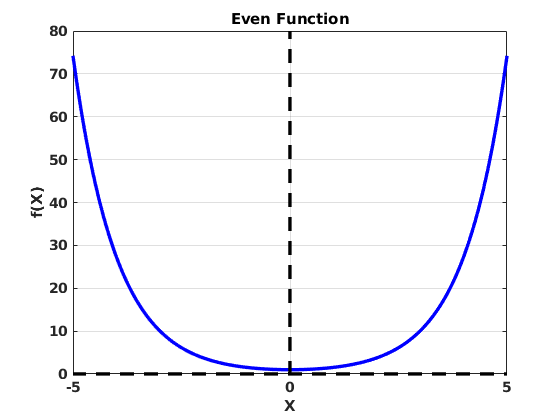
\includegraphics{lec16_even.png}
\caption{An example even function.}
\label{fig:even-fun}
\end{marginfigure}
\begin{marginfigure}
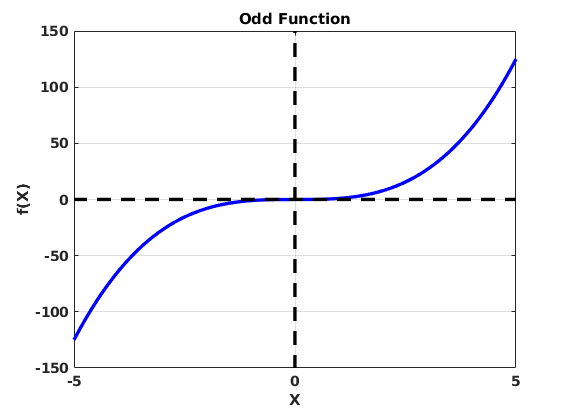
\includegraphics{lec16_odd.png}
\caption{An example odd function.}
\label{fig:odd-fun}
\end{marginfigure}
\begin{definition}[Even Function]
A function is even if, for all real values $x$, $f(-x) = f(x)$.  
\end{definition}
An example of an even function is shown in Figure \ref{fig:even-fun}.
\begin{definition}[Odd Function]
A function is odd if, for all real values $x$, $f(-x) = -f(x)$.
\end{definition}
An example of an odd function is shown in Figure \ref{fig:odd-fun}.

\newthought{Some properties} of even an odd functions include:\sidenote{Students are welcome to prove these assertions.}
\begin{enumerate}
\item An even function times an even function results in an even function.
\item An odd function times an odd function results in an even function.
\item An even function times an odd function results in an odd function.
\item Adding or subtracting two even functions results in an even function.
\item Adding or subtracting two odd functions results in an odd function.
\item $\int_{-p}^{p} f_{\text{even}}(x) \ dx = 2\int_{0}^{p} f_{\text{even}}(x) \ dx$ and $\int_{-p}^{p} f_{\text{odd}}(x) \ dx = 0$.
\end{enumerate}

The ``even-ness'' or ``odd-ness'' of a function is relevant to Fourier series expansions.  If you expand an \emph{even} function in a Fourier series you will find that all of the $b_n$ coefficients are zero.  If you expand an \emph{odd} function in a Fourier series you will find that $a_0$ and $a_n$ terms are all zero.

You can still use the formulas presented in Equation \ref{eq:Fourier-Coeff} when expanding even or odd functions.  Alternatively, you can use the formulas for the Cosine expansion or Sine expansion below for even or odd functions respectively.

\vspace{0.5cm}

\noindent\textbf{Cosine series:}\marginnote{The cosine and sine series expansions are sometimes referred to as ``half-wave'' expansions since the calculations, as shown in the formulas, only involve the portion of the wave in the interval [0,p]---the positive half-wave.}
\begin{align}
\begin{split}
f(x) &= \frac{a_0}{2} + \sum\limits_{n=1}^{\infty}a_n \cos{\frac{n \pi x}{p}} \\
a_0 &= \frac{2}{p}\int_0^p \ f(x) \ dx \\
a_n &= \frac{2}{p} \int_0^p \ f(x) \cos{\frac{n \pi x}{p}} \ dx
\end{split}
\end{align}

\vspace{0.5cm}

\noindent\textbf{Sine series:}
\begin{align}
\begin{split}
f(x) &= \sum\limits_{n=1}^{\infty} b_n \sin{\frac{n \pi x}{p}} \\
b_n &= \frac{2}{p}\int_{0}^{p} \ f(x) \ \sin{\frac{n \pi x}{p}} \ dx
\end{split}
\end{align}

